% Ibrahimbegovic, Taylor & Wilson (1990)
% "A robust quadrilateral membrane finite element with drilling degrees of freedom"
% Int. J. Numer. Methods Eng., 30, 445-457.
% Formulas extraidas del PDF. Figuras recortadas en fig/*.png
\documentclass[11pt]{article}
\usepackage[utf8]{inputenc}
\usepackage[spanish]{babel}
\usepackage{amsmath,amssymb,graphicx,booktabs,geometry}
\geometry{margin=2.5cm}
\newcommand{\symm}{\operatorname{symm}}
\newcommand{\skewop}{\operatorname{skew}}
\begin{document}
\title{ITW 1990 --- membrana cuadrilatera con GDL de giro (drilling)}
\author{Ibrahimbegovic, Taylor \& Wilson --- IJNME 30:445--457}
\date{}\maketitle

\section{Problema de contorno}
Para todo $\mathbf{x}\in\Omega$:
\begin{align}
\operatorname{div}\boldsymbol\sigma + \mathbf f &= \mathbf 0 \tag{1}\\
\skewop\boldsymbol\sigma &= \mathbf 0 \tag{2}\\
\boldsymbol\psi &= \skewop\nabla\mathbf u \tag{3}\\
\symm\boldsymbol\sigma &= \mathbf C\cdot\symm\nabla\mathbf u \tag{4}
\end{align}
Descomposicion euclidiana:
\begin{equation}
\boldsymbol\sigma=\symm\boldsymbol\sigma+\skewop\boldsymbol\sigma,\quad
\symm\boldsymbol\sigma=\tfrac12(\boldsymbol\sigma+\boldsymbol\sigma^{T}),\quad
\skewop\boldsymbol\sigma=\tfrac12(\boldsymbol\sigma-\boldsymbol\sigma^{T})
\tag{5--7}
\end{equation}
Constitutiva isotropa en tension plana:
\begin{equation}
C_{ijkl}=\lambda\,\delta_{ij}\delta_{kl}+\mu(\delta_{ik}\delta_{jl}+\delta_{il}\delta_{jk}),
\qquad i,j,k,l\in\{1,2\}
\tag{8}
\end{equation}
\begin{equation}
\lambda=\frac{\nu E}{1-\nu^{2}},\qquad \mu=\frac{E}{2(1+\nu)}
\tag{9,10}
\end{equation}

\section{Formulaciones variacionales}
\textbf{Problema (M)} --- mixto, con $\skewop\boldsymbol\tau$ como multiplicador de Lagrange:
\begin{multline}
\Pi_{\gamma}(\mathbf v,\boldsymbol\omega,\skewop\boldsymbol\tau)=
\tfrac12\int_{\Omega}\symm(\nabla\mathbf v)\cdot\mathbf C\cdot(\symm\nabla\mathbf v)\,d\Omega
+\int_{\Omega}\skewop\boldsymbol\tau^{T}\cdot(\skewop\nabla\mathbf v-\boldsymbol\omega)\,d\Omega\\
-\tfrac12\gamma^{-1}\int_{\Omega}|\skewop\boldsymbol\tau|^{2}d\Omega
-\int_{\Omega}\mathbf v\cdot\mathbf f\,d\Omega
\tag{11}
\end{multline}
Sustituyendo $\gamma^{-1}\skewop\boldsymbol\sigma=\skewop\nabla\mathbf u-\boldsymbol\psi$ (13) se obtiene el

\noindent\textbf{Problema (D)} --- penalizacion en desplazamientos:
\begin{equation}
\tilde\Pi_{\gamma}(\mathbf v,\boldsymbol\omega)=
\tfrac12\int_{\Omega}\symm(\nabla\mathbf v)\cdot\mathbf C\cdot(\symm\nabla\mathbf v)\,d\Omega
+\tfrac12\gamma\int_{\Omega}|\skewop\nabla\mathbf v-\boldsymbol\omega|^{2}d\Omega
-\int_{\Omega}\mathbf v\cdot\mathbf f\,d\Omega
\tag{14}
\end{equation}
\begin{multline}
0=\int_{\Omega}(\symm\nabla\mathbf v)\cdot\mathbf C\cdot(\symm\nabla\mathbf u)\,d\Omega
+\gamma\int_{\Omega}(\skewop\nabla\mathbf v-\boldsymbol\omega)^{T}\cdot(\skewop\nabla\mathbf u-\boldsymbol\psi)\,d\Omega\\
-\int_{\Omega}\mathbf v\cdot\mathbf f\,d\Omega
\tag{15}
\end{multline}

\paragraph{Sobre $\gamma$ (literal del paper).}
Hughes \emph{et al.} sugieren tomar $\gamma$ igual al modulo de cortante, $\gamma=\mu$.
Pero los autores anaden: \emph{``the numerical studies we have performed have shown that
the formulation is insensitive to the value of $\gamma$ used (at least for several orders
of magnitude which bound the shear modulus)''}. La Tabla V lo mide: de $\gamma/\mu=0.001$
a $1000$ el resultado cambia en la quinta cifra.

\section{Interpolacion (elemento de 4 nudos)}
Giro independiente, bilineal:
\begin{equation}
u_{3}\equiv\psi^{h}=\sum_{e}\sum_{I=1}^{4}N_{I}^{e}(r,s)\,\psi_{I},
\qquad N_{I}^{e}=\tfrac14(1+r_{I}r)(1+s_{I}s)
\tag{17,18}
\end{equation}
Desplazamiento tipo Allman + burbuja jerarquica:
\begin{equation}
\mathbf u^{h}=\sum_{e}\sum_{I=1}^{4}N_{I}^{e}\mathbf u_{I}
+\sum_{e}\sum_{I=5}^{8}NS_{I}^{e}(r,s)\,\frac{l_{JK}}{8}(\psi_{K}-\psi_{J})\,\mathbf n_{JK}
+\sum_{e}NB_{9}^{e}(r,s)\,\Delta\mathbf u_{9}
\tag{19}
\end{equation}
con $\mathbf n_{JK}=\{\cos\alpha_{JK};\sin\alpha_{JK}\}$ la normal exterior del lado y
$l_{JK}=\big((x_{K1}-x_{J1})^{2}+(x_{K2}-x_{J2})^{2}\big)^{1/2}$ (20),
$J=I-4$, $K=\mathrm{mod}(I,4)+1$ (21). Funciones serendipity y burbuja:
\begin{align}
NS_{I}^{e}&=\tfrac12(1-r^{2})(1+s_{I}s), & I&=5,7 \tag{22}\\
NS_{I}^{e}&=\tfrac12(1+r_{I}r)(1-s^{2}), & I&=6,8 \tag{23}\\
NB_{9}^{e}&=(1-r^{2})(1-s^{2}) &&\tag{24}
\end{align}
La burbuja se \textbf{condensa estaticamente} a nivel de elemento.
El campo de tension antisimetrica es \textbf{constante} por elemento:
$\skewop\tau^{h}=\sum_{e}\tau_{0}^{e}$ (25).

\subsection{Matrices $\mathbf B$ y $\mathbf G$}
\begin{equation}
\symm\nabla\mathbf u^{e}=\mathbf B_{I}^{e}\mathbf u_{I}+\mathbf G_{I}^{e}\psi_{I},
\qquad
\mathbf B_{I}^{e}=\begin{bmatrix} N^{e}_{I,x_{1}} & 0\\ 0 & N^{e}_{I,x_{2}}\\ N^{e}_{I,x_{2}} & N^{e}_{I,x_{1}}\end{bmatrix}
\tag{26,27}
\end{equation}
\begin{equation}
\mathbf G_{I}^{e}=\frac18
\begin{bmatrix}
l_{IJ}\cos\alpha_{IJ}NS^{e}_{L,x_{1}}-l_{IK}\cos\alpha_{IK}NS^{e}_{M,x_{1}}\\[2pt]
l_{IJ}\sin\alpha_{IJ}NS^{e}_{L,x_{2}}-l_{IK}\sin\alpha_{IK}NS^{e}_{M,x_{2}}\\[2pt]
\big(l_{IJ}\cos\alpha_{IJ}NS^{e}_{L,x_{2}}-l_{IK}\cos\alpha_{IK}NS^{e}_{M,x_{2}}\big)
+\big(l_{IJ}\sin\alpha_{IJ}NS^{e}_{L,x_{1}}-l_{IK}\sin\alpha_{IK}NS^{e}_{M,x_{1}}\big)
\end{bmatrix}
\tag{28}
\end{equation}
con los indices (estilo FORTRAN)
\begin{equation}
I=1,2,3,4;\quad M=I+4;\quad L=M-1+4\,\mathrm{aint}(1/I);\quad K=\mathrm{mod}(M,4)+1;\quad J=L-4
\tag{29}
\end{equation}

\subsection{Residuo del drilling}
\begin{equation}
\skewop\nabla\mathbf u^{e}-\psi^{e}=\mathbf b_{I}^{e}\mathbf u_{I}+g_{I}^{e}\psi_{I}
\tag{30}
\end{equation}
\begin{equation}
\mathbf b_{I}^{e}=\big\langle -\tfrac12 N^{e}_{I,x_{2}}\;;\;\tfrac12 N^{e}_{I,x_{1}}\big\rangle,
\qquad I=1,2,3,4
\tag{31}
\end{equation}
\begin{multline}
g_{I}^{e}=\Big[-\tfrac{1}{16}\big(l_{IJ}\cos\alpha_{IJ}NS^{e}_{L,x_{2}}-l_{IK}\cos\alpha_{IK}NS^{e}_{M,x_{2}}\big)\\
+\tfrac{1}{16}\big(l_{IJ}\sin\alpha_{IJ}NS^{e}_{L,x_{1}}-l_{IK}\sin\alpha_{IK}NS^{e}_{M,x_{1}}\big)-N_{I}^{e}\Big]
\tag{32}
\end{multline}

\section{Matrices de rigidez}
Parte constitutiva (comun a las dos formulaciones):
\begin{equation}
\mathbf K^{e}=\int_{\Omega^{e}}[\mathbf B^{e}\;\;\mathbf G^{e}]^{T}\,\mathbf C\,[\mathbf B^{e}\;\;\mathbf G^{e}]\,d\Omega
\tag{33}
\end{equation}
\begin{equation}
\mathbf h^{e}=\int_{\Omega^{e}}\langle \mathbf b^{e};\mathbf g^{e}\rangle^{T}d\Omega
\tag{34}
\end{equation}
\textbf{Mixta (M-type)} --- sistema y condensacion de $\tau_{0}^{e}$:
\begin{equation}
\begin{bmatrix}\mathbf K^{e} & \mathbf h^{e}\\ \mathbf h^{eT} & -\gamma^{-1}\Omega^{e}\end{bmatrix}
\begin{Bmatrix}\mathbf a\\ \tau_{0}^{e}\end{Bmatrix}
=\begin{Bmatrix}\mathbf f\\ 0\end{Bmatrix},
\qquad \mathbf a=\begin{Bmatrix}\mathbf u\\ \boldsymbol\psi\end{Bmatrix}
\tag{35}
\end{equation}
\begin{equation}
\boxed{\;\hat{\mathbf K}^{e}=\mathbf K^{e}+\frac{\gamma}{\Omega^{e}}\,\mathbf h^{e}\mathbf h^{eT}\;}
\tag{36}
\end{equation}
\textbf{Desplazamientos (D-type)} --- penalizacion directa:
\begin{equation}
\mathbf P^{e}=\gamma\int_{\Omega^{e}}\begin{Bmatrix}\mathbf b^{e}\\ \mathbf g^{e}\end{Bmatrix}
\langle \mathbf b^{e};\mathbf g^{e}\rangle\,d\Omega
\tag{38}
\end{equation}
\begin{equation}
\boxed{\;[\mathbf K^{e}+\mathbf P^{e}]\,\mathbf a=\mathbf f\;}
\tag{39}
\end{equation}

\paragraph{Integracion (la clave practica).}
$\mathbf K^{e}$ y $\mathbf h^{e}$ con \textbf{Gauss $3\times3$}; $\mathbf P^{e}$ con
\textbf{UN solo punto}. Integrando $\mathbf K^{e}$ completo y sumando $\mathbf P^{e}$
(o $\gamma\,\mathbf h^{e}\mathbf h^{eT}/\Omega^{e}$) \emph{no quedan modos de energia nula}
y no hace falta ningun otro artificio (nada de control de reloj de arena a la
MacNeal--Harder). El teorema de equivalencia de Malkus--Hughes hace que la integracion
reducida selectiva (39) sea equivalente a la mixta (36); la unica diferencia viene de la
burbuja, que \emph{no} contribuye a $\mathbf P^{e}$ pero si a
$\mathbf h^{e}\mathbf h^{eT}$, y solo se nota en elementos distorsionados.

\paragraph{Para la cascara.} La membrana se combina con la placa \textbf{DKQ}. Para que
la membrana no bloquee se aplica la modificacion de Taylor y se usa la regla de
\textbf{8 puntos} sobre $\mathbf K^{e}$. La correccion de Jetteur para elemento alabeado
no hace falta.

\section{Solucion exacta del cantilever (Timoshenko--Goodier)}
\begin{equation}
u_{2}=\frac{Pl^{3}}{3EI}+\frac{(4+5\nu)Pl}{2Eh}=0.3553
\tag{Fig.\,4}
\end{equation}

\section{Casos y resultados de referencia}
\begin{center}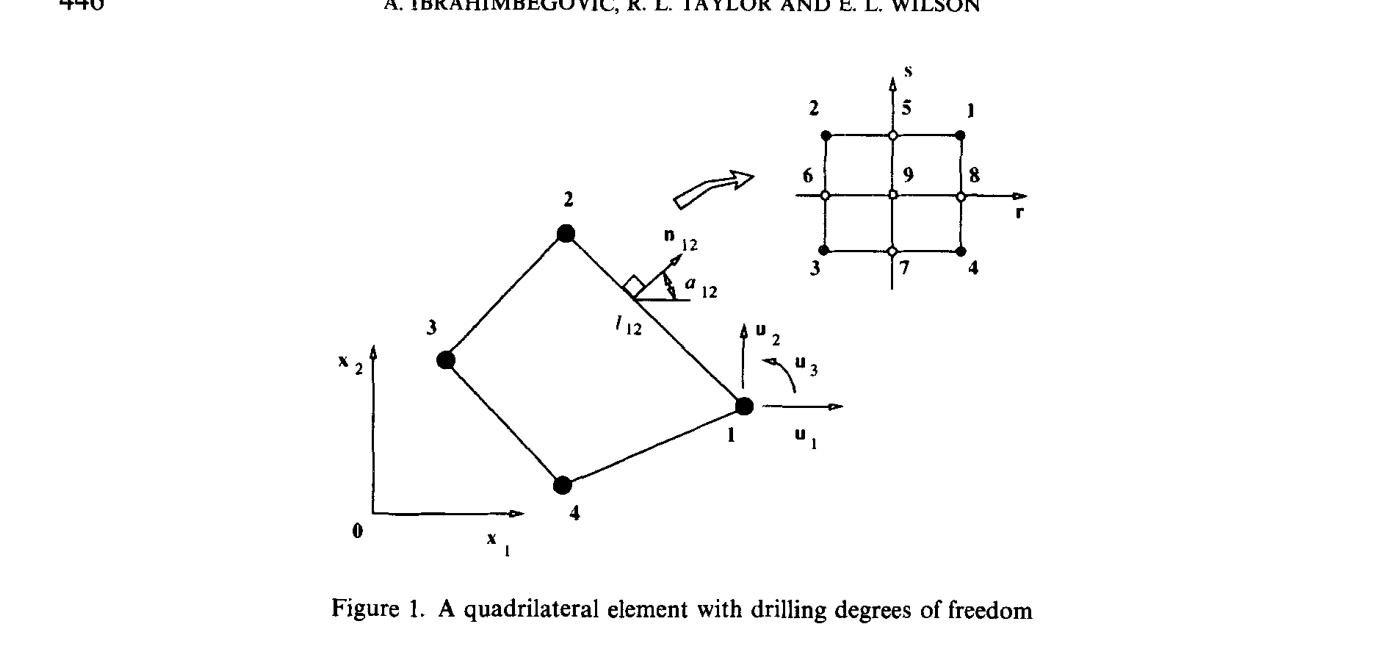
\includegraphics[width=.85\textwidth]{fig/fig1_elemento_drilling.png}\end{center}
\begin{center}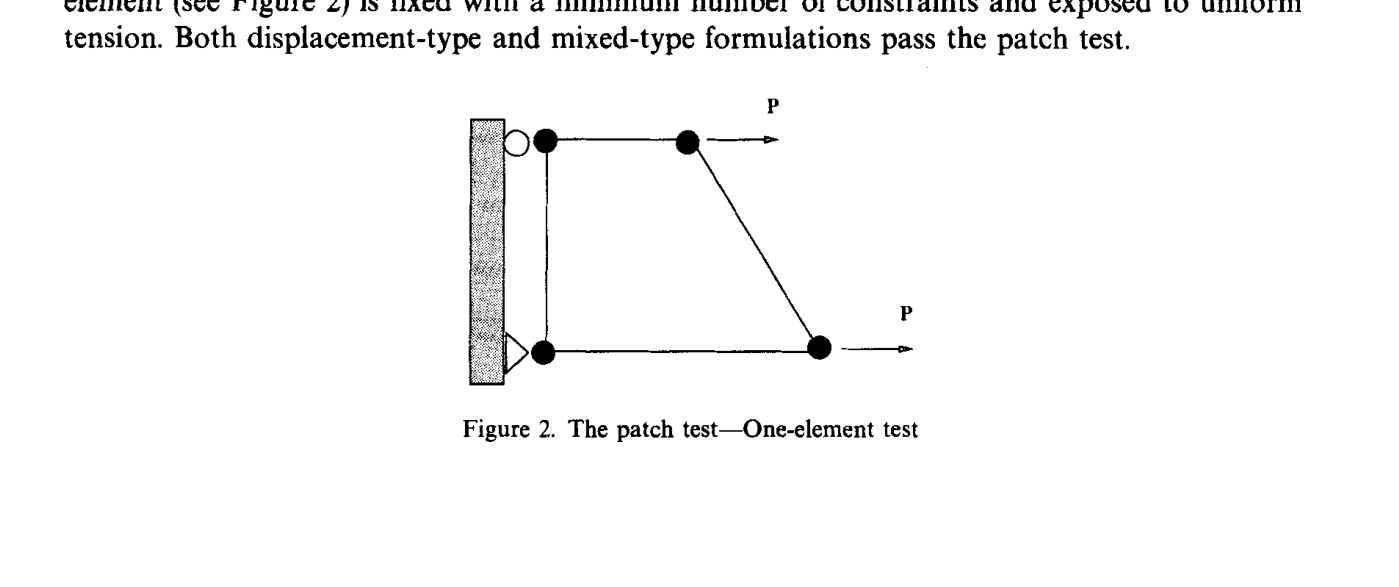
\includegraphics[width=.6\textwidth]{fig/fig2_patch_test.png}\end{center}
\begin{center}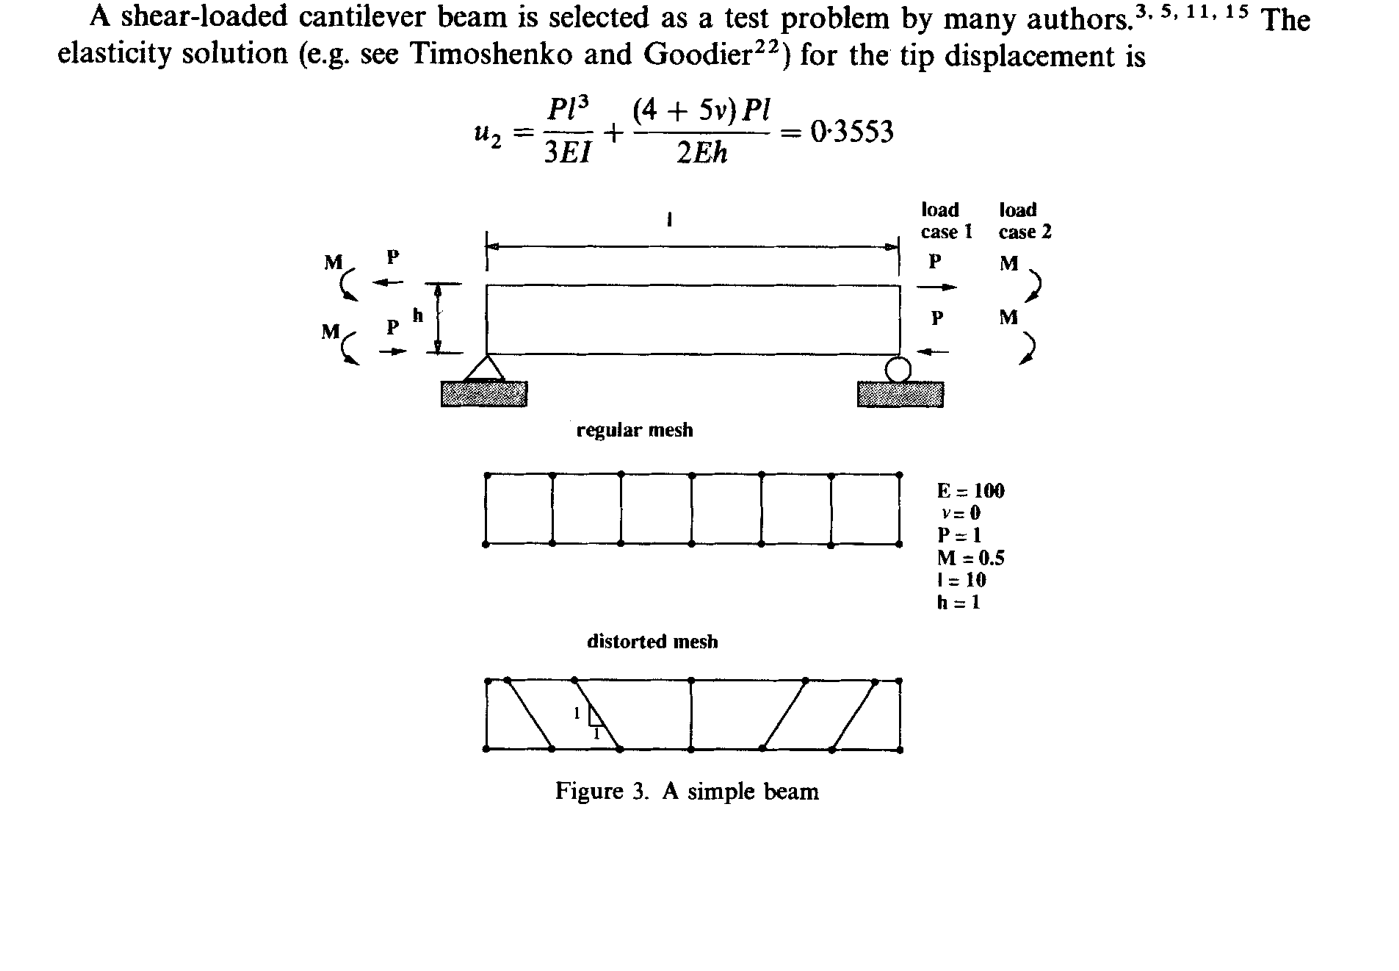
\includegraphics[width=.85\textwidth]{fig/fig3_viga_simple.png}\end{center}
\begin{center}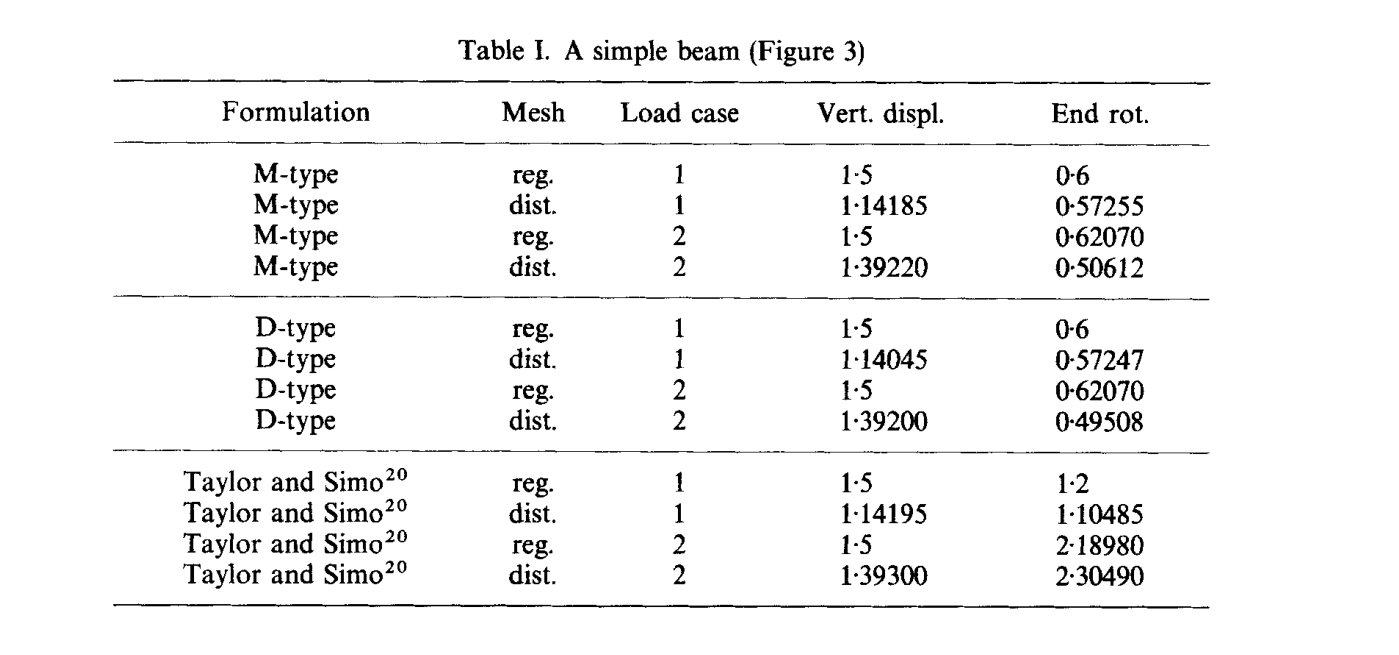
\includegraphics[width=.85\textwidth]{fig/tabla1_viga_simple.png}\end{center}
\begin{center}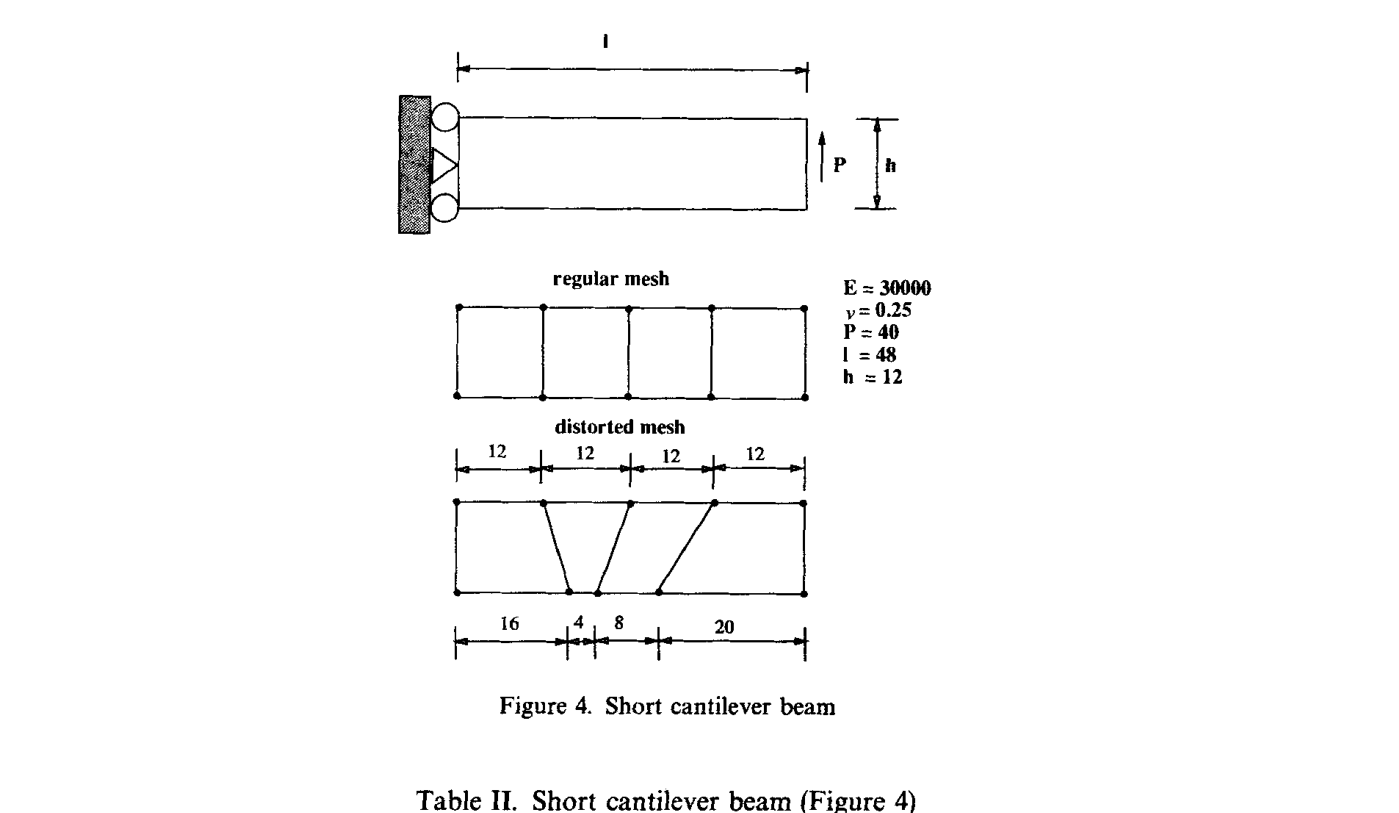
\includegraphics[width=.85\textwidth]{fig/fig4_cantilever_corto.png}\end{center}
\begin{center}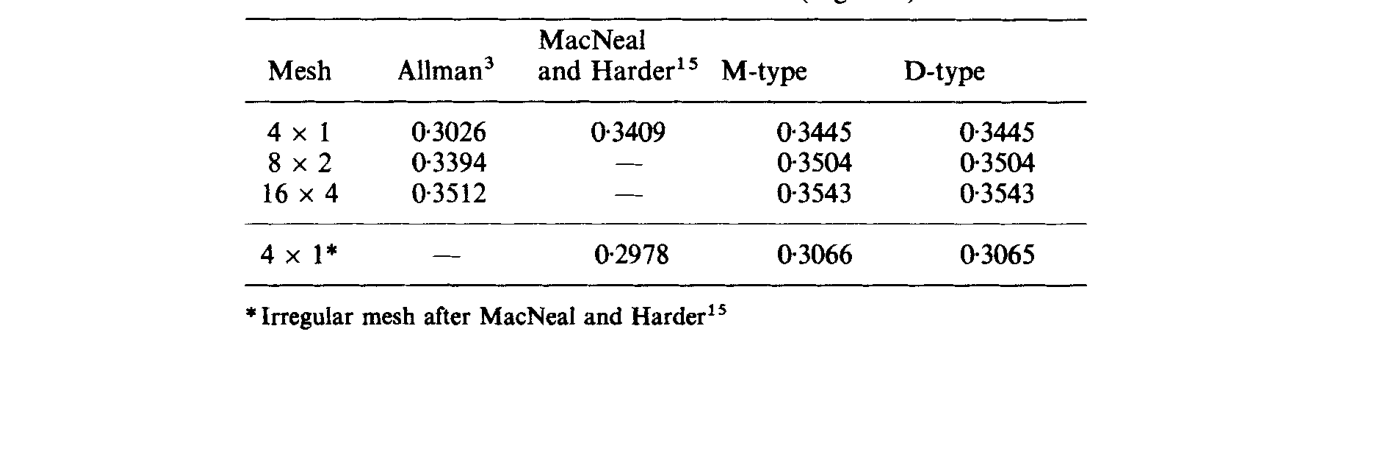
\includegraphics[width=.85\textwidth]{fig/tabla2_cantilever.png}\end{center}
\begin{center}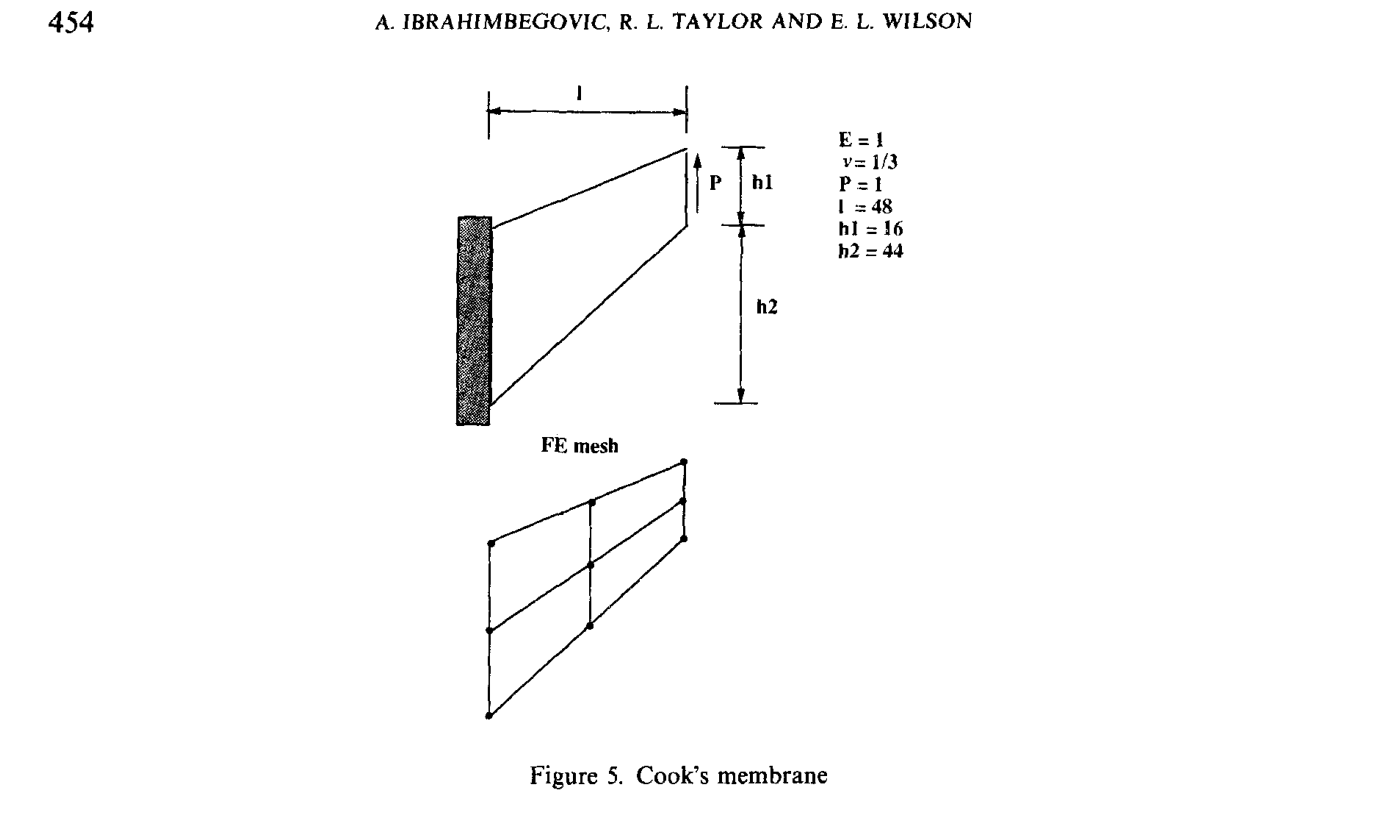
\includegraphics[width=.7\textwidth]{fig/fig5_cook.png}\end{center}
\begin{center}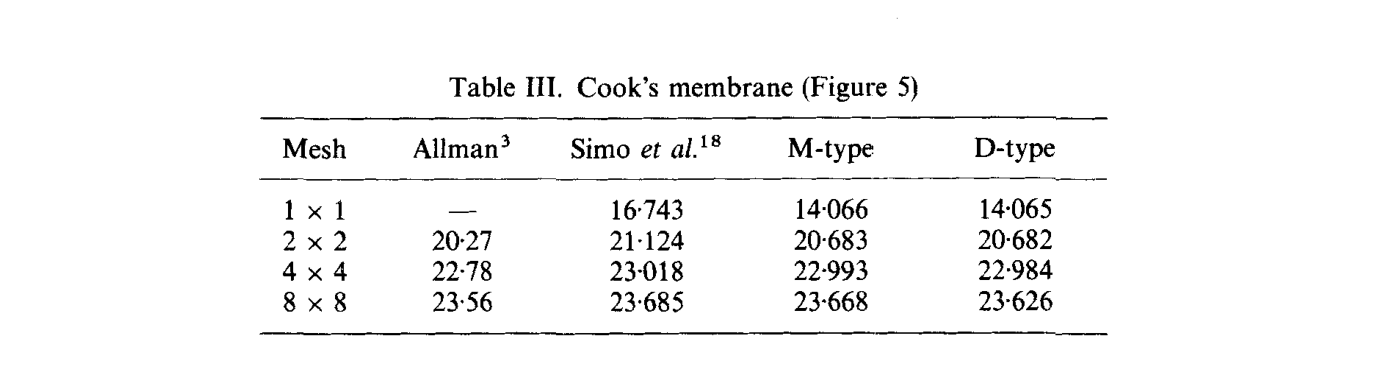
\includegraphics[width=.85\textwidth]{fig/tabla3_cook.png}\end{center}
\begin{center}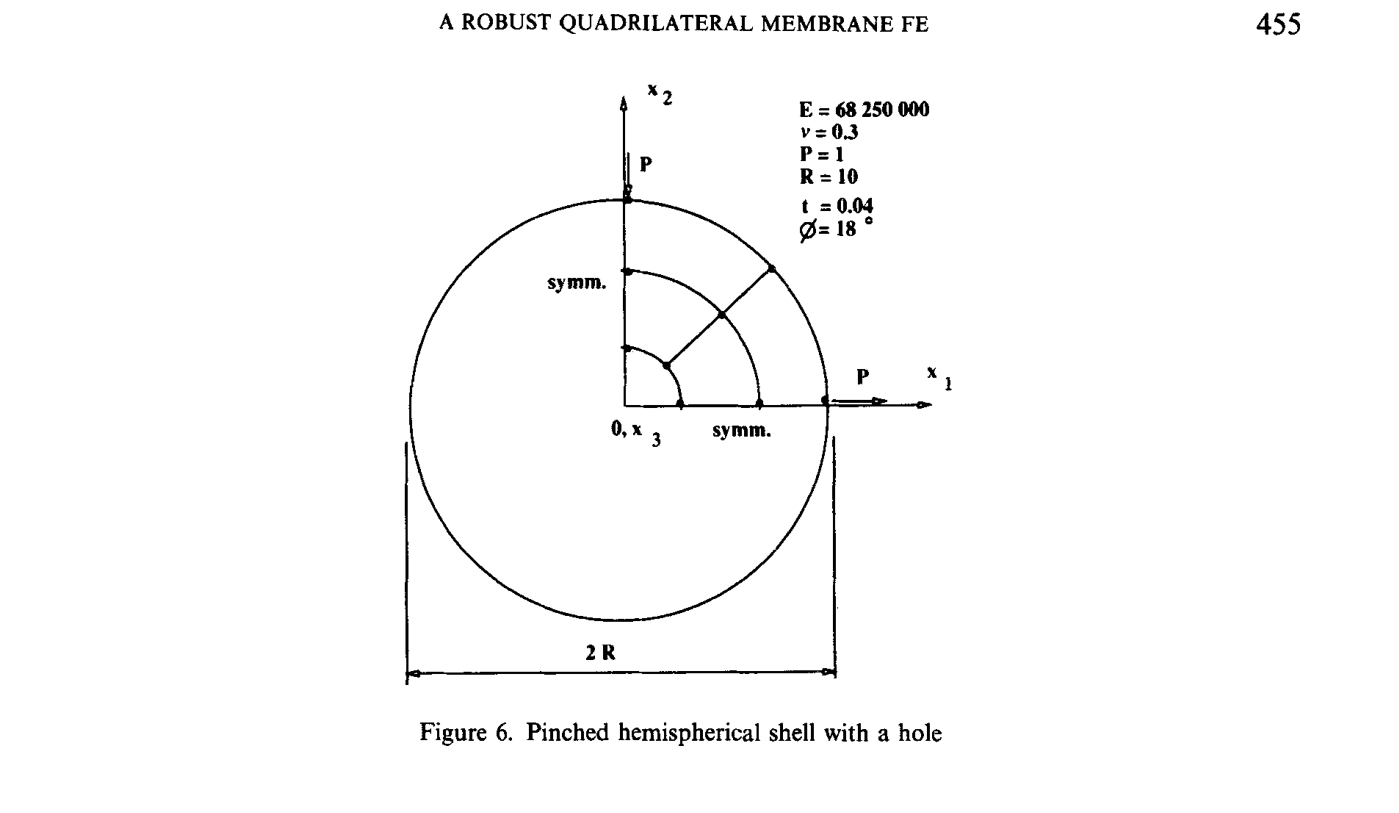
\includegraphics[width=.7\textwidth]{fig/fig6_hemisferio.png}\end{center}
\begin{center}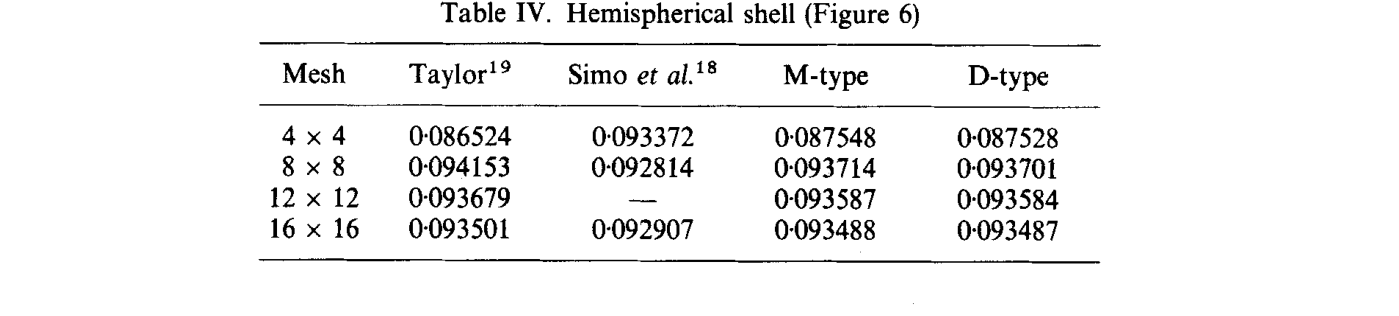
\includegraphics[width=.85\textwidth]{fig/tabla4_hemisferio.png}\end{center}
\begin{center}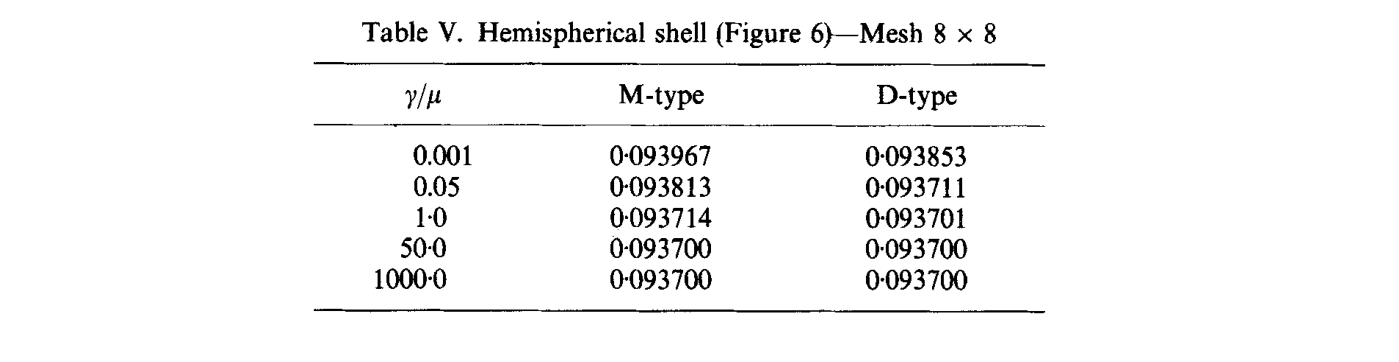
\includegraphics[width=.7\textwidth]{fig/tabla5_gamma.png}\end{center}
\end{document}
